\chapter{Detection Transformer}
\label{sec:detr}

The previous chapter showed that heatmap regression performs well for GW searches. However, the approach is limited by the time resolution of the output heatmap, which becomes problematic for close overlaps. One possible solution would be to increase the heatmap resolution, for example by adding \emph{upsampling} steps after the transformer encoder, similar to U-Net architectures \cite{ronneberger2015unetconvolutionalnetworksbiomedical}.

In this chapter, a different approach is investigated, forgoing the heatmap representation entirely. Instead, a fully end-to-end model is developed: for a given sample, the model directly outputs multiple GW candidates, each with a signal score and time location. The approach is based on the Detection Transformer (DETR) \cite{10.1007/978-3-030-58452-8_13}, which was originally developed for object detection in images and is modified here to handle time-series data instead. Although not implemented in this thesis, such a model could also be adapted to return estimates of signal parameters, which is important for low-latency searches.

\section{Architecture and Training}

\begin{figure}
	\centering
	\makebox[\textwidth]{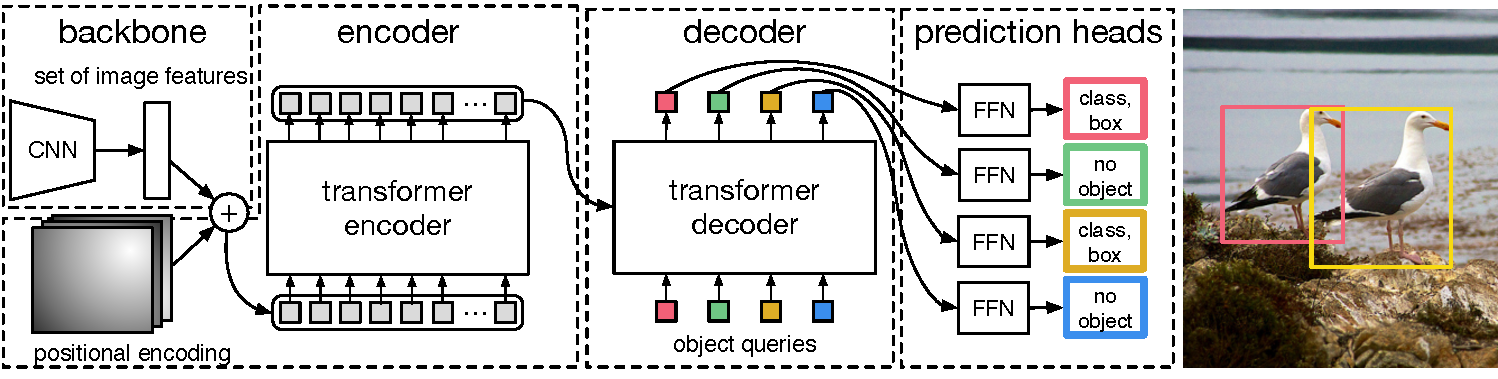
\includegraphics[width=16cm]{multiple_signal_detection/images/DETR_detail_seagulls}}
	\caption{Original DETR~\cite{10.1007/978-3-030-58452-8_13} architecture for image object detection. The model outputs multiple object class scores and bounding boxes.}
	\label{fig:detr:detr}
\end{figure}

The DETR architecture consists of a CNN backbone, a transformer encoder, and a transformer decoder. Up to the encoder, the architecture is similar to the transformer-based heatmap regressor from the previous chapter. The difference is that the encoder output tokens are not read out directly to produce a heatmap, but serve as the source sequence of a transformer decoder. The decoder takes a number of learned \emph{queries} as its target sequence. Each decoder output is then read out via two prediction heads to produce a class score and a signal coalescence time. In principle, by appending more prediction heads, this architecture can be adapted to return other parameters as well. See a schematic of the original DETR architecture in Fig.~\ref{fig:detr:detr}. In this sense, DETR can be viewed as extending the classification-token idea of ViTs~\cite{DBLP:journals/corr/abs-2010-11929} to multiple learned prediction queries.

One limitation of the DETR architecture is that the number of possible predictions per sample is fixed by the query count. In practice, this is handled by choosing the number of queries sufficiently large.

\begin{figure}
	\centering
	\makebox[\textwidth]{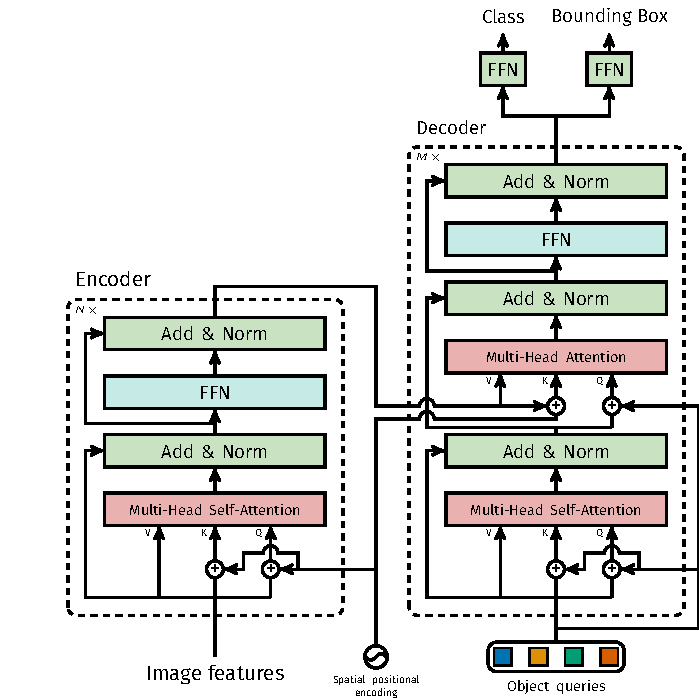
\includegraphics[width=10cm]{multiple_signal_detection/images/transformer}}
	\caption{Detailed implementation of the transformer used in DETR~\cite{10.1007/978-3-030-58452-8_13}. Positional encodings are not applied before the value projections.}
	\label{fig:detr:transformer}
\end{figure}

For the CNN backbone, the same ResNet model as previously is employed. Given samples with a length of \SI{64}{\second}, the backbone outputs $512$ vectors of size $256$. A convolution operation with kernel size one projects these onto the embedding dimension $d_\text{embed}=64$. Both the transformer encoder and decoder consist of six layers and eight heads, and employ FFNs with hidden dimension $d_\text{ff}=1024$. A dropout probability of \SI{10}{\percent} is used throughout the model. The transformer employs sinusoidal encodings for the encoder tokens and learned embeddings for the queries. Following the original DETR architecture, these are applied before the query and key projections only, not before the value projections (see Fig.~\ref{fig:detr:transformer}).

A number of $m=16$ queries is chosen. For the higher ET event-rate estimate of $\lambda=\SI{1e6}{\per\year}$, the probability for more than $16$ signals in a $T=\SI{64}{\second}$ sample is negligible:
\begin{equation}
	P(n>16) =
	1-\sum_{k=0}^{16}
	\frac{(\lambda T)^k}{k!}\exp[-\lambda T]
	= \SI{7e-9}{\percent}.
\end{equation}
Thus, $16$ queries are more than sufficient for the expected signal multiplicities considered here. These queries are learnable parameters of size $d_\text{embed}$, initialized as zero and optimized together with the rest of the network. After being passed through the decoder, each query is read out via two prediction heads.

The class score is obtained through
\begin{align}
	n &= \mathrm{LayerNorm}(x),\\
	h &= \mathrm{Dropout}(\mathrm{ReLU}(\mathrm{Linear}_{64\rightarrow1024}(n))),\\
	z_c &= \mathrm{Dropout}(\mathrm{Linear}_{1024\rightarrow1}(h)),
\end{align}
which is later passed through a sigmoid layer,
\begin{equation}
	\hat c = \mathrm{Sigmoid}(z_c).
\end{equation}
For the time prediction, the prediction head reads
\begin{align}
	n &= \mathrm{LayerNorm}(x),\\
	h_1 &= \mathrm{Dropout}(\mathrm{ReLU}(\mathrm{Linear}_{64\rightarrow1024}(n))),\\
	h_2 &= \mathrm{Dropout}(\mathrm{ReLU}(\mathrm{Linear}_{1024\rightarrow1024}(h_1))),\\
	h_3 &= \mathrm{Dropout}(\mathrm{ReLU}(\mathrm{Linear}_{1024\rightarrow1024}(h_2))),\\
	z_t &= \mathrm{Dropout}(\mathrm{Linear}_{1024\rightarrow1}(h_3)).
\end{align}
This value is also passed through a sigmoid layer to normalize the prediction to $[0,1]$ in units of total sample time,
\begin{equation}
	\hat t = \mathrm{Sigmoid}(z_t).
\end{equation}
In total, the network has \SI{6.2}{\mega\nothing} trainable parameters.

For any given sample, the DETR architecture implemented here produces $m=16$ predictions,
\begin{equation}
	\hat y = \{(\hat c_j,\hat t_j)\}_{j=1}^{m},
\end{equation}
each comprising a signal score and coalescence time. The network is free to output predictions with $\hat c_j\approx0$, which are interpreted as no-signal predictions and discarded after thresholding. The class score and time prediction are trained in tandem, employing a BCE loss and an $L_1$ loss summed over all predictions:
\begin{equation}
	\pazocal{L}(y,\hat y)
	=
	\sum_{j=1}^{m}
	\pazocal{L}_\text{BCE}(c_j,\hat c_j)
	+
	c_j\,\lambda |t'_j-\hat t_j|.
	\label{eq:detr:loss}
\end{equation}
For predictions corresponding to a no-signal ground truth, $c_j=0$, the time-prediction loss is zeroed out. Since for random class predictions the average BCE loss is $\pazocal{L}_\text{BCE}=\ln 2\approx0.69$, while the matched $L_1$ loss is of order $10^{-2}$, the $L_1$ term is up-weighted. The exact value $\lambda=6$ is chosen empirically.

It remains to define how the ground truth $y=\{(c_j,t'_j)\}_{j=1}^{m}$ corresponding to the $m$ predictions is constructed. For this, all signals $\{t_i\}_{i=1}^{n}$, where $n<m$, are assigned to predictions by a matching algorithm. Then the ground truth $y=\{y_j\}_{j=1}^{m}$ is constructed with
\begin{equation}
	\label{eq:detr:ground_truth}
	y_j = \begin{cases}
		(1, t_i) & \text{if signal $i$ is matched to prediction $j$,} \\
		(0, \varnothing) & \text{otherwise.}
	\end{cases}
\end{equation}
For unmatched predictions, the ground-truth coalescence time does not matter, as the corresponding $L_1$ loss is zeroed out.

Following \cite{10.1007/978-3-030-58452-8_13}, signals $i$ and predictions $j$ are matched by minimizing the cost
\begin{equation}
	\pazocal{L}_\text{cost}(t_i,\hat y_j)
	=
	-\hat c_j + \lambda|t_i-\hat t_j|,
\end{equation}
where again $\lambda=6$. Let $\tau:\pazocal{I}\rightarrow\pazocal{J}'$ denote an \emph{assignment function} mapping the signal indices $\pazocal{I}=\{1,2,\dots,n\}$ to a subset of all prediction indices $\pazocal{J}'\subset\pazocal{J}=\{1,2,\dots,m\}$. The \emph{optimal} assignment function $\pi$ is the realization of $\tau$ that minimizes the total assignment cost over all signals $i$ and corresponding predictions $\tau(i)$:
\begin{equation}
	\pi
	=
	\operatorname*{arg\,min}_{\tau}
	\sum_{i=1}^{n}
	\pazocal{L}_\text{cost}(t_i,\hat y_{\tau(i)}).
\end{equation}
This is an \emph{assignment problem}, which is solved using methods implemented by SciPy~\cite{2020SciPy-NMeth}.

The index $i$ of the signal matched to prediction $j$ is given by $\pi^{-1}(j)$. This inverse is only defined for matched predictions, $j\in\pazocal{J}'$. Thus, with Eq.~\ref{eq:detr:ground_truth}, the ground truth $y_j$ corresponding to prediction $\hat y_j$ can be written as
\begin{equation}
	y_j = \begin{cases}
		(1, t_{\pi^{-1}(j)}) & \text{if $j\in\pazocal{J}'$,} \\
		(0, \varnothing) & \text{otherwise.}
	\end{cases}
\end{equation}

The model is trained on the same \SI{1}{\mega\nothing}-sample training dataset as the heatmap regressors and evaluated on the corresponding \SI{131}{\kilo\nothing}-sample test dataset. The AdamW optimizer is used with a learning rate of $10^{-4}$, a weight decay of $10^{-4}$, and a batch size of $64$. Training is performed for a maximum of $100$ epochs. The checkpoint with the lowest validation loss is used for evaluation.

\begin{figure}
	\centering
	\makebox[\textwidth]{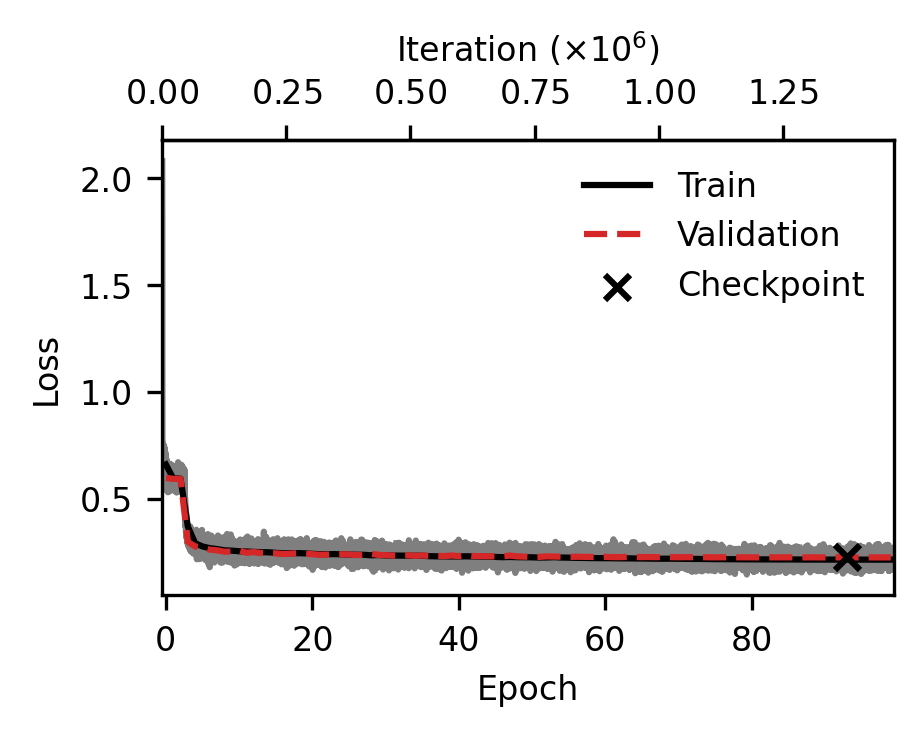
\includegraphics[width=9cm]{multiple_signal_detection/plots/learning_curves/detr_loss}}
	\caption{Learning curve of the DETR model. The training loss is shown per step and averaged over each epoch. The validation loss is shown in red, and the marker denotes the minimum validation loss used for checkpoint selection.}
	\label{fig:detr:learning_curve}
\end{figure}

The learning curve is shown in Fig.~\ref{fig:detr:learning_curve}. The validation loss reaches its minimum after $0$ epochs. After this point, the model begins to overfit. Therefore, the minimum-validation-loss checkpoint is used for all following results.

\section{Comparison with Heatmap Regression}

The following results and discussion largely mirror the structure of the previous chapter. The DETR model is evaluated with the same detection-ratio/FAR metrics and the same matching tolerance as the heatmap regressors. The difference is that DETR directly outputs candidate scores and times, so no peak extraction or local soft-argmax post-processing is required.

It is again useful to first inspect individual model outputs. Figure~\ref{fig:detr:out} shows five representative examples. The DETR model produces meaningful GW candidates, and applying a class-score threshold of \SI{69}{\percent} retrieves most visible signals while keeping the number of FPs limited. The choice of this threshold corresponds to the fixed operating point discussed below. The predicted coalescence times also appear sufficiently accurate for the matching criterion used in this work.

In contrast to heatmap regression, the DETR predictions are produced by individual queries. These queries interact with the encoded time series through cross-attention. The examples in Fig.~\ref{fig:detr:out} indicate that individual queries assign most of their attention to localized regions of the input, often close to the corresponding signal coalescence time. This supports the interpretation that the queries act as signal-candidate slots, although the attention weights should only be understood as a diagnostic of the model behavior.

\begin{figure}
	\centering
	\makebox[\textwidth]{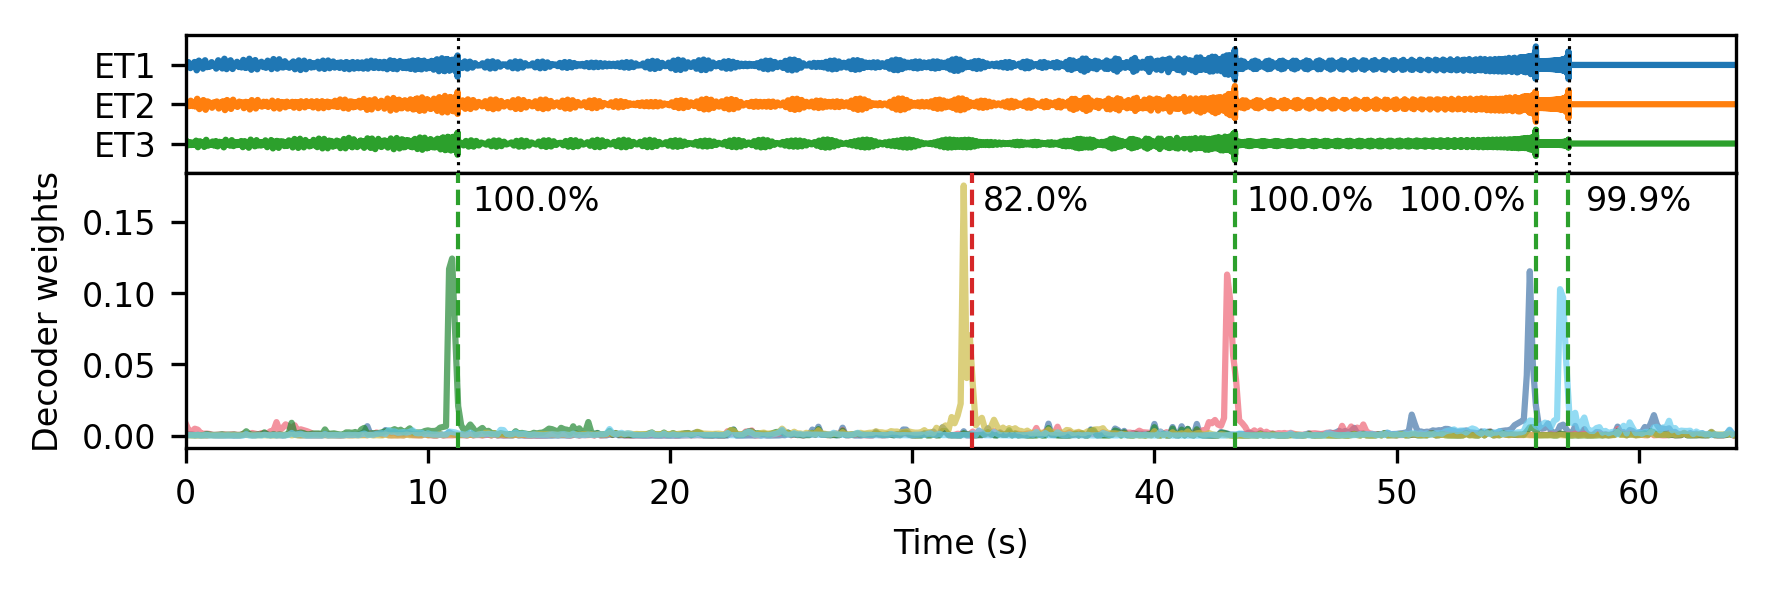
\includegraphics[width=15cm]{multiple_signal_detection/plots/out/300/detr/0}}
	\makebox[\textwidth]{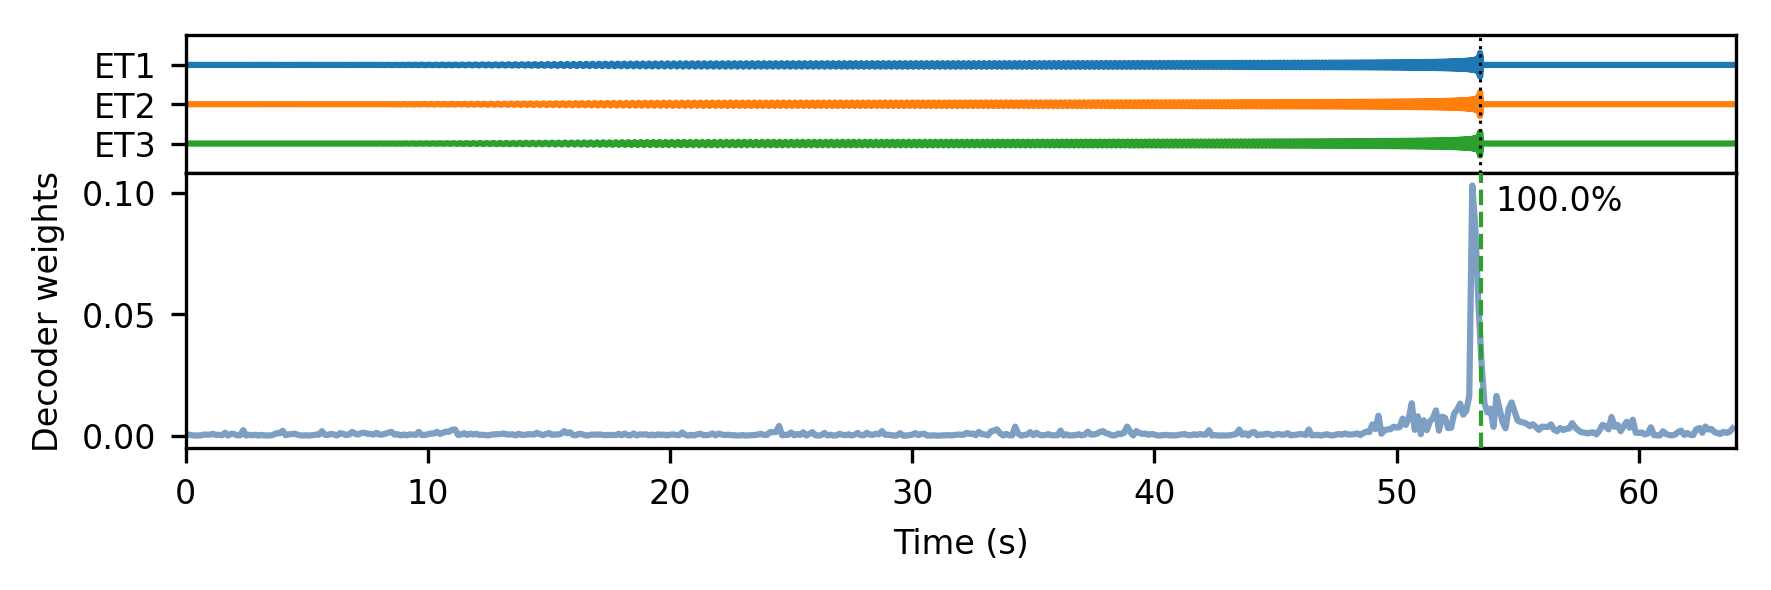
\includegraphics[width=15cm]{multiple_signal_detection/plots/out/300/detr/1}}
	\makebox[\textwidth]{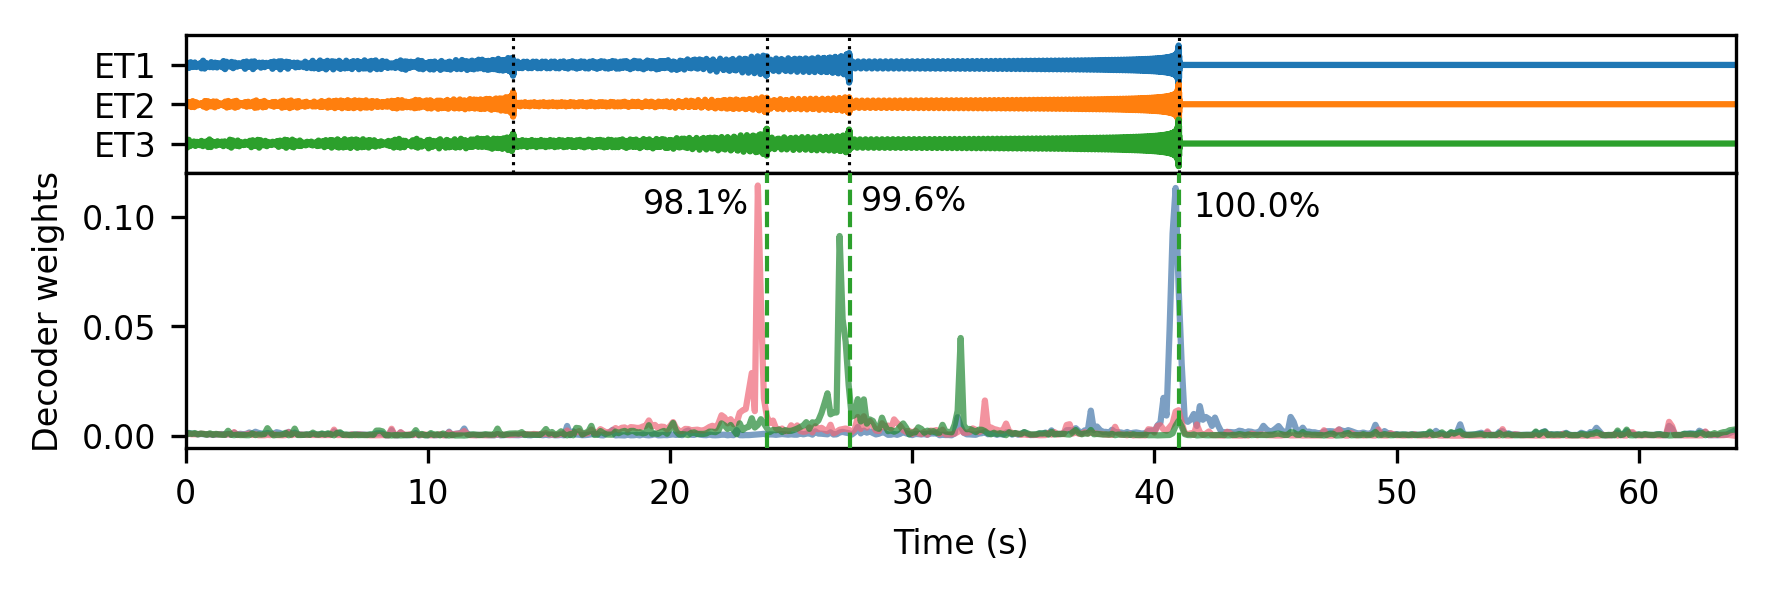
\includegraphics[width=15cm]{multiple_signal_detection/plots/out/300/detr/2}}
	\makebox[\textwidth]{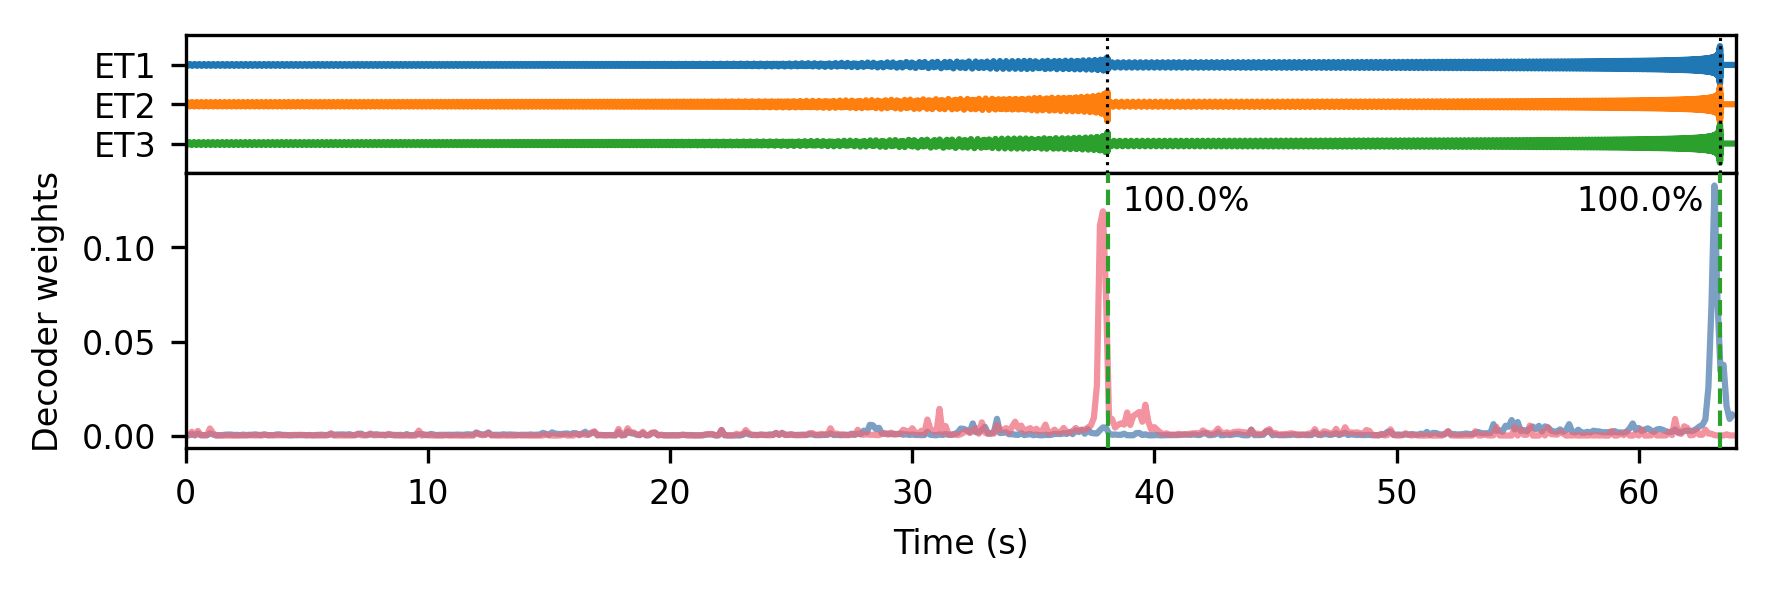
\includegraphics[width=15cm]{multiple_signal_detection/plots/out/300/detr/3}}
	\makebox[\textwidth]{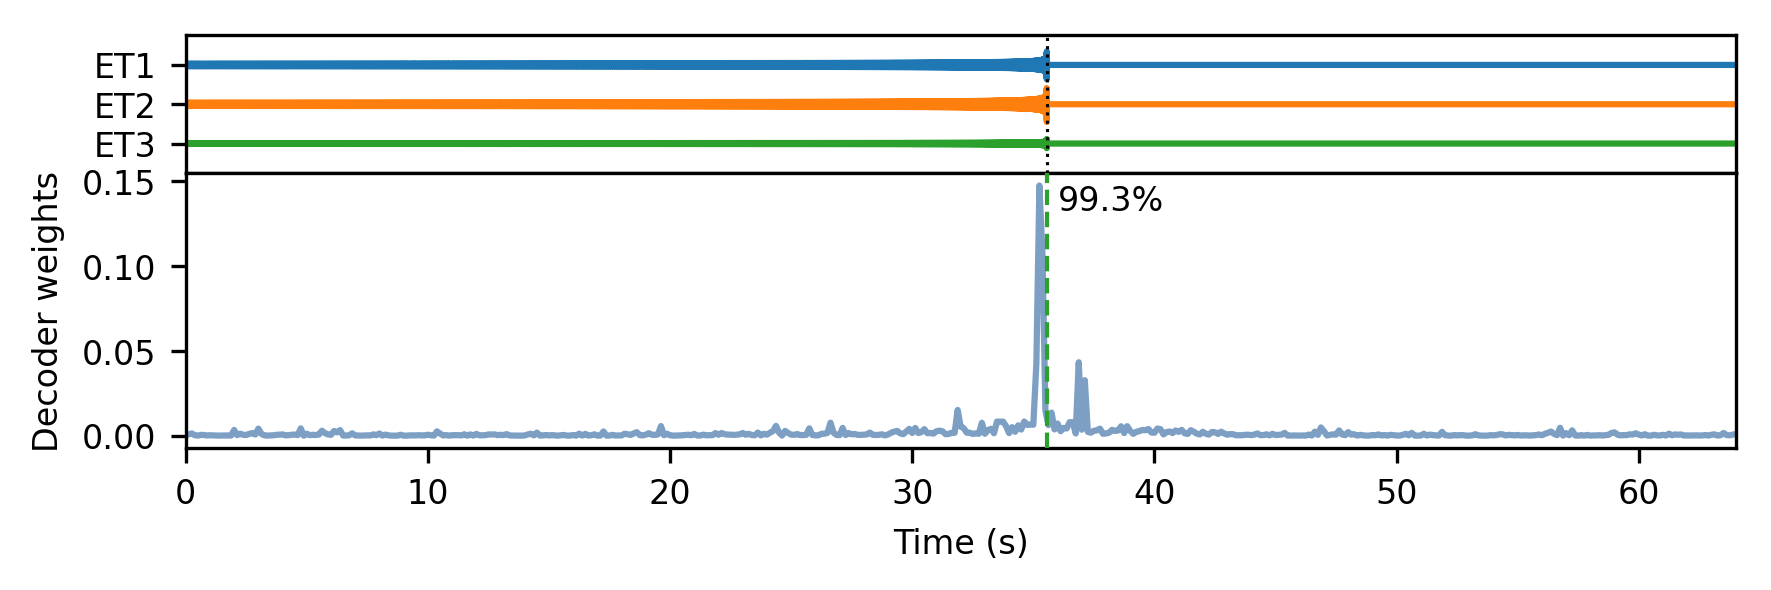
\includegraphics[width=15cm]{multiple_signal_detection/plots/out/300/detr/4}}
	\caption{Example DETR predictions for five test samples. Predictions above a score threshold of \SI{69}{\percent} are shown as GW candidates. For each candidate, the predicted coalescence time and class score are indicated.}
	\label{fig:detr:out}
\end{figure}

A quantitative comparison is obtained by varying the score threshold and computing the detection ratio and FAR over the full test dataset. Figure~\ref{fig:detr:far} compares the resulting operating characteristic of DETR with the CNN and transformer-encoder heatmap regressors from the previous chapter. Over a large part of the FAR range, DETR performs comparably to the transformer heatmap model. In the intermediate FAR regime, between \SI{0}{\per\second} and \SI{0}{\per\second}, DETR even reaches a higher detection ratio. At the lowest FARs, however, DETR falls below the heatmap regressors. This suggests that the direct set-prediction approach produces useful candidates, but its score ranking or calibration is less robust in the extreme low-FAR regime.

At the fixed operating point $1/(10\,\mathrm{min})$, DETR reaches a detection ratio of \SI{0}{\percent}, compared to \SI{0}{\percent} for the CNN heatmap regressor and \SI{0}{\percent} for the transformer-encoder heatmap regressor. The corresponding score threshold is \SI{0}{\percent}. Thus, DETR achieves comparable performance to heatmap regression while removing the need for heatmap peak extraction.

\begin{figure}
	\centering
	\makebox[\textwidth]{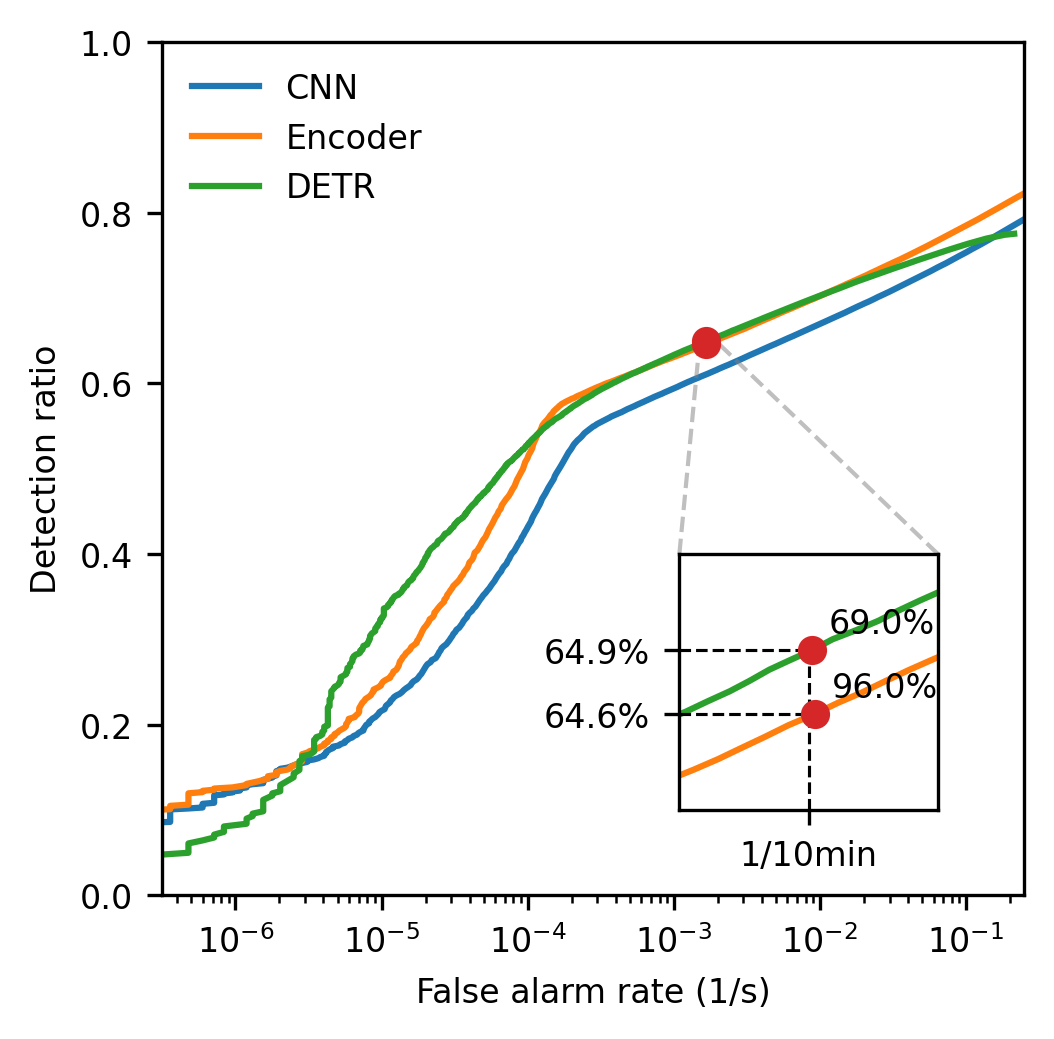
\includegraphics[width=9cm]{multiple_signal_detection/plots/cnn_encoder_detr_far}}
	\caption{Detection ratio as a function of FAR for the CNN heatmap regressor, transformer-encoder heatmap regressor, and DETR model. All models are evaluated on the same test set using the same matching criterion. DETR directly outputs candidate times and scores, while the heatmap models require peak extraction.}
	\label{fig:detr:far}
\end{figure}

The dependence on the number of signals per sample is shown in Fig.~\ref{fig:detr:num_mergers}. Similar to the transformer heatmap regressor, DETR improves for larger $n$. This suggests that the model benefits from the presence of multiple signal-containing regions in the input, consistent with the use of global attention. The behavior differs from the CNN heatmap model, whose performance remains approximately constant with $n$. Quantitatively, the DETR detection ratio changes from \SI{0}{\percent} for $n=1$ to \SI{0}{\percent} for $n=6$.

\begin{figure}
	\centering
	\makebox[\textwidth]{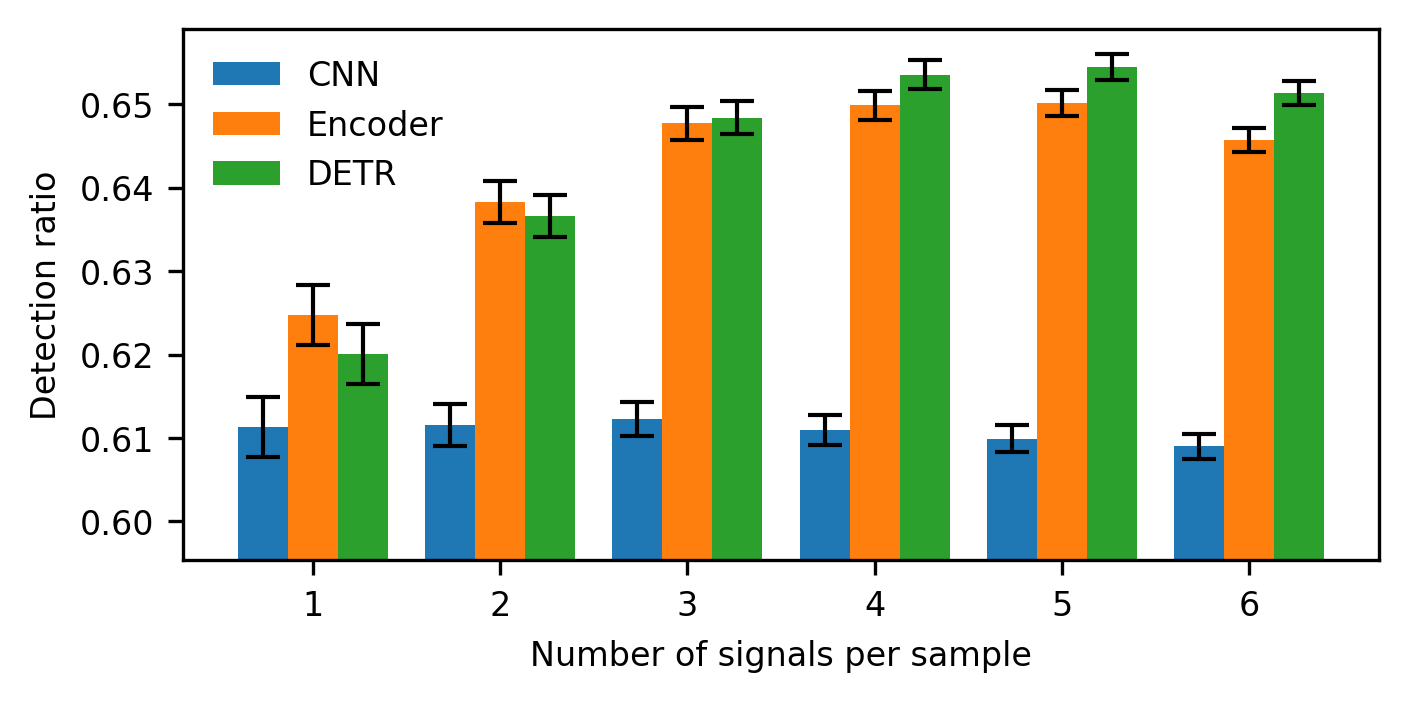
\includegraphics[width=12cm]{multiple_signal_detection/plots/cnn_encoder_detr_mergers}}
	\caption{Detection ratio as a function of the number of signals per \SI{64}{\second} sample for the CNN heatmap regressor, transformer-encoder heatmap regressor, and DETR model. The fixed operating point corresponds to a FAR of $1/(10\,\mathrm{min})$.}
	\label{fig:detr:num_mergers}
\end{figure}

An important difference between DETR and heatmap regression is the way coalescence times are predicted. In heatmap regression, the model predicts a fixed-resolution time series and the final coalescence time is obtained through peak extraction and a local soft-argmax. In DETR, the time is predicted directly as a continuous output of the corresponding query. This should improve the time-localization accuracy.

To test this, the time residual
\begin{equation}
	\Delta t = \hat t - t
\end{equation}
is computed for true-positive predictions at the fixed operating point. The residuals are converted from normalized sample units to seconds. The result for DETR and the corresponding result for the transformer heatmap regressor are shown in Fig.~\ref{fig:detr:time_acc}. DETR achieves a mean residual of \SI{0}{\second} and a standard deviation of \SI{0}{\second}, compared to \SI{0}{\second} and \SI{0}{\second} for the heatmap model. Thus, DETR improves the time-localization accuracy, as expected from its direct time-regression output.

\begin{figure}
	\centering
	\makebox[\textwidth][c]{%
		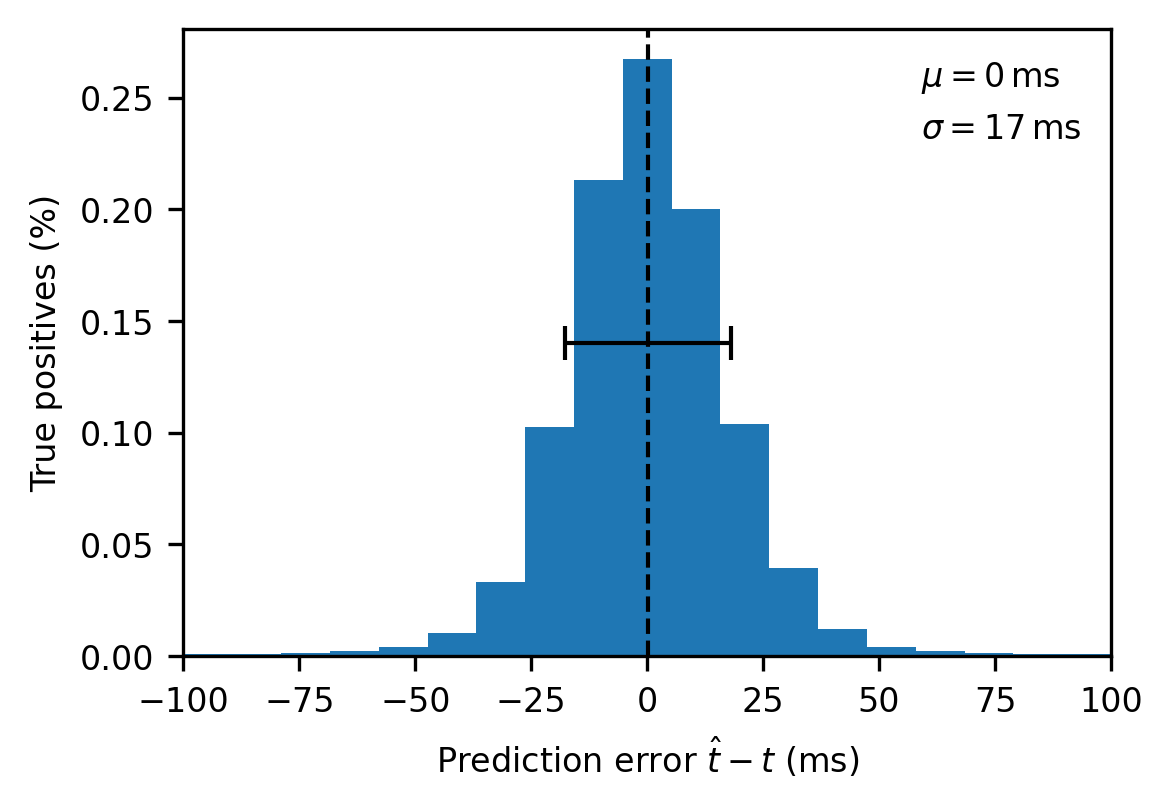
\includegraphics[width=8cm]{multiple_signal_detection/plots/detr_time}
		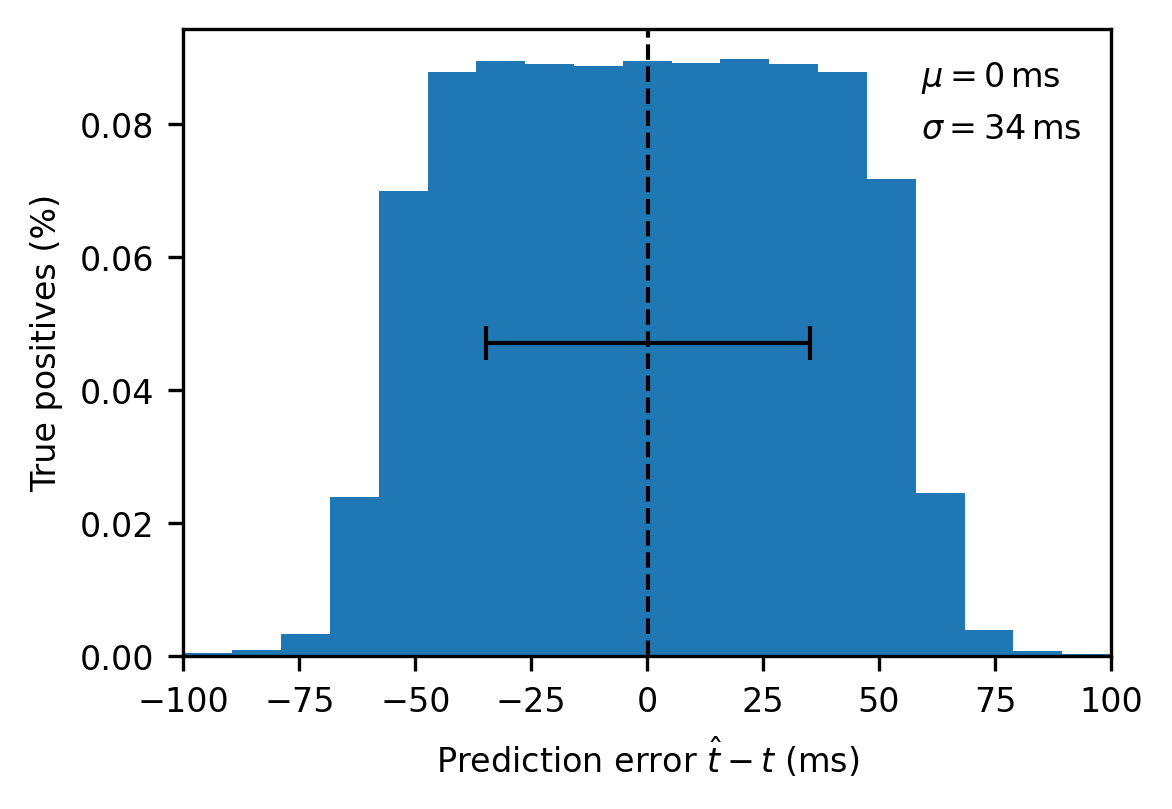
\includegraphics[width=8cm]{multiple_signal_detection/plots/encoder_time}
	}
	\caption{Time-localization residuals $\Delta t=\hat t-t$ for true-positive predictions at the fixed operating point. The left plot shows DETR predictions, and the right plot shows transformer heatmap-regressor predictions. Times are shown in seconds.}
	\label{fig:detr:time_acc}
\end{figure}

\section{Injection Study}

The previous chapter showed that heatmap regression becomes limited for very close signal separations, where two nearby heatmap peaks can no longer be cleanly resolved. Since DETR predicts coalescence times directly, it is not limited by the fixed time resolution of a heatmap in the same way. Therefore, one may expect improved performance for close overlaps. To test this, the same two-signal injection study as in the previous chapter is repeated for DETR.

Figure~\ref{fig:detr:deltat} shows the detection ratio as a function of coalescence-time separation. DETR does not show the same explicit heatmap-resolution cutoff as the heatmap model. However, close overlaps remain challenging. The detection ratio stays approximately constant for $\Delta t_\text{coa}\gtrsim\SI{0}{\second}$, and decreases for smaller separations. Compared to the transformer heatmap regressor, DETR is comparable in this study. This indicates that direct time regression removes the fixed heatmap-grid limitation, but does not make close-overlap detection trivial.

\begin{figure}
	\centering
	\makebox[\textwidth]{
		\includegraphics[width=12cm]{multiple_signal_detection/plots/encoder_detr_stacked}
	}
	\caption{Detection ratio as a function of coalescence-time separation $\Delta t_\text{coa}$ for the transformer heatmap regressor and DETR. Each sample contains two signals with fixed separation.}
	\label{fig:detr:deltat}
\end{figure}

A more detailed view is obtained by distinguishing four recovery cases: only the earlier signal A is recovered, only the later signal B is recovered, both signals are recovered, or neither signal is recovered. The result is shown in Fig.~\ref{fig:detr:deltat_cases}, together with the corresponding heatmap-regression result. DETR can still output two distinct candidates for small separations, but the fraction of samples where both signals are recovered decreases in the close-overlap regime. Instead, single-signal recoveries become more common. This suggests that the remaining difficulty is not the time resolution of the output representation, but the reliable assignment of two high-confidence queries to two nearby signals.

\begin{figure}
	\centering
	\makebox[\textwidth]{
		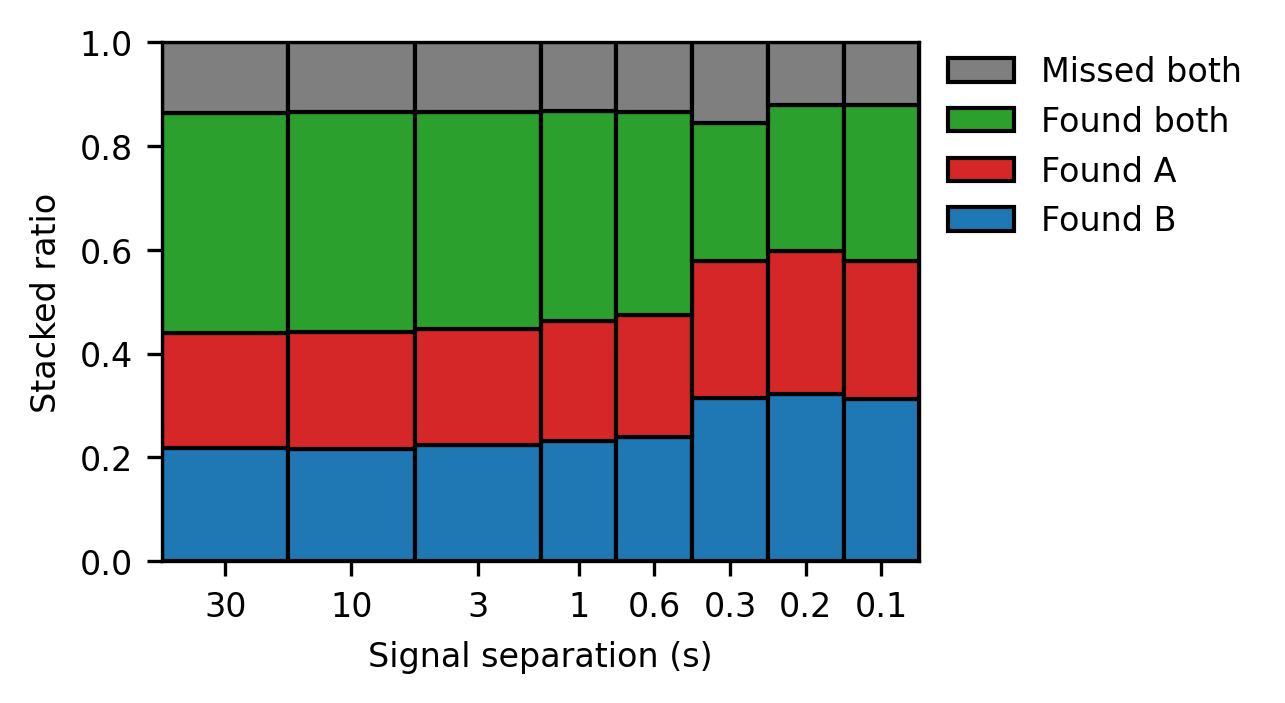
\includegraphics[
		height=6cm, 
		trim=0 0 3cm 0,
		clip]{multiple_signal_detection/plots/detr_stacked}
		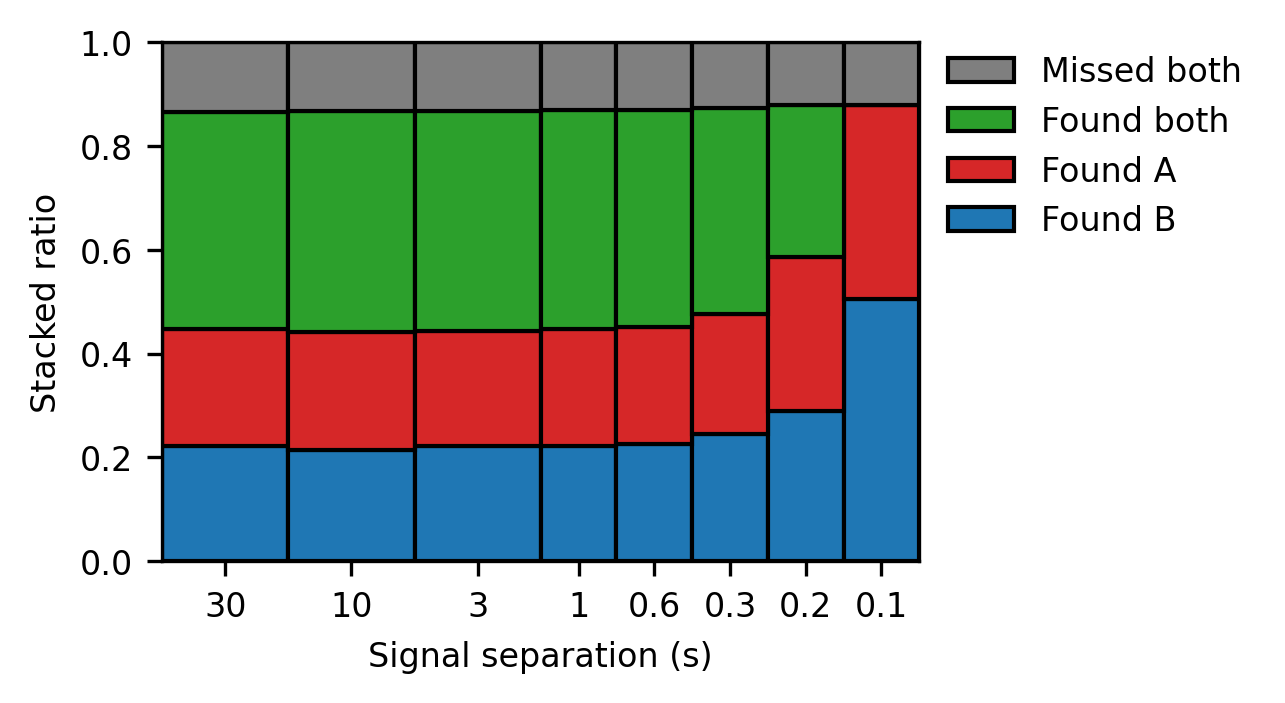
\includegraphics[
		height=6cm, 
		trim=1cm 0 0 0,
		clip]{multiple_signal_detection/plots/encoder_stacked}
	}
	\caption{Recovery cases as a function of coalescence-time separation for DETR and the transformer heatmap regressor. Each sample is categorized according to whether only signal A, only signal B, both signals, or neither signal is recovered.}
	\label{fig:detr:deltat_cases}
\end{figure}

The qualitative behavior can also be seen in individual close-overlap examples, shown in Fig.~\ref{fig:detr:deltat_plot}. DETR can place separate predictions at small time separations without relying on a fixed-resolution heatmap grid. This supports the interpretation that the remaining performance loss is not caused by an explicit output-grid resolution. Instead, close overlaps remain difficult because the model must assign separate high-confidence queries to signals with very similar coalescence times.

\begin{figure}
	\centering
	\makebox[\textwidth]{
		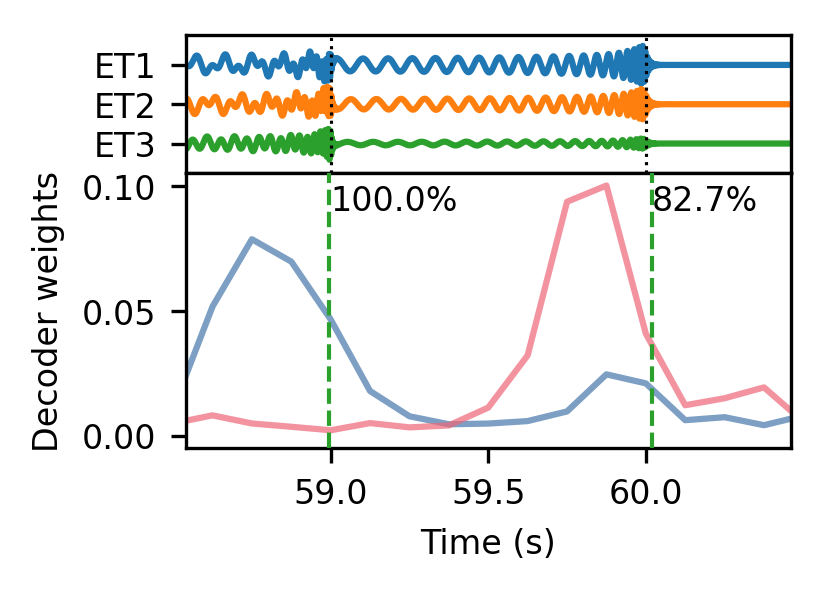
\includegraphics[
		height=5cm,
		trim=0 0 0 0,
		clip
		]{multiple_signal_detection/plots/out/700/detr/0_zoom}
		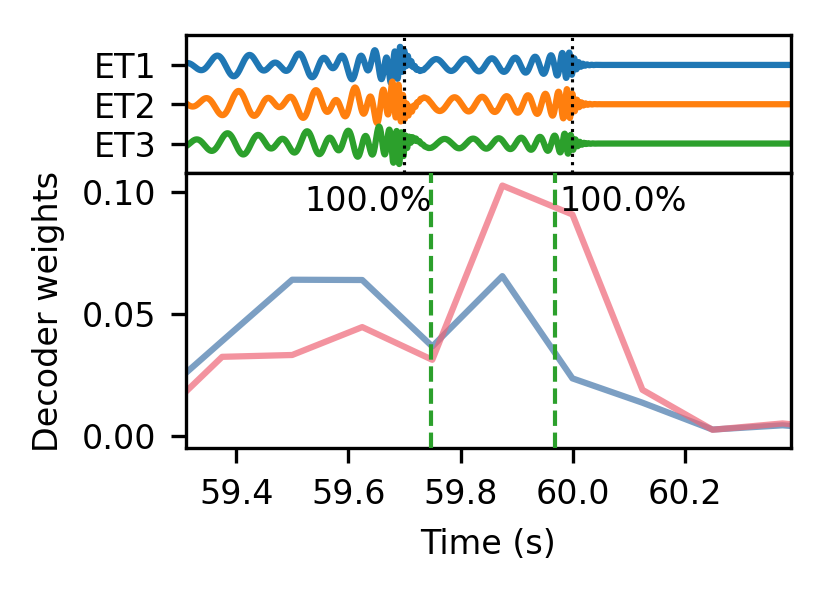
\includegraphics[
		height=5cm,
		trim=1.35cm 0 0 0,
		clip
		]{multiple_signal_detection/plots/out/800/detr/7_zoom}
		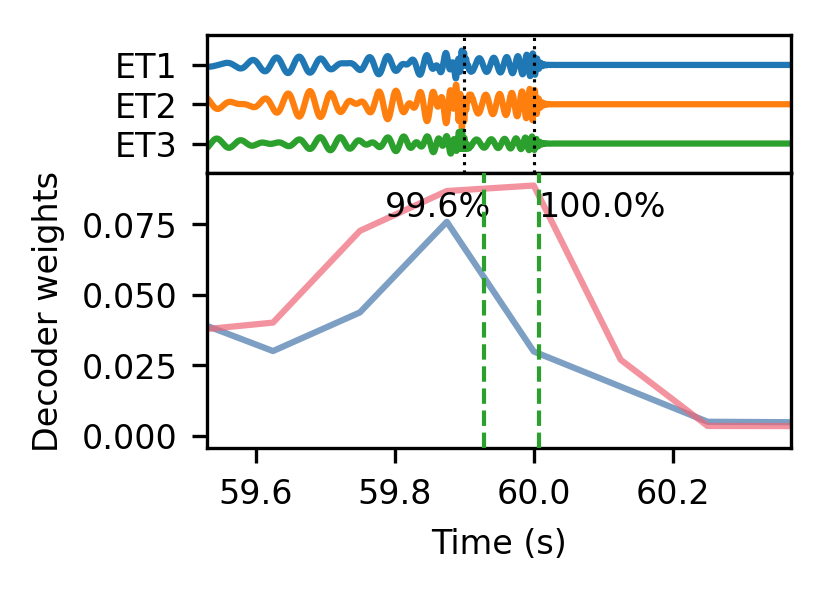
\includegraphics[
		height=5cm,
		trim=1.35cm 0 0 0,
		clip
		]{multiple_signal_detection/plots/out/900/detr/6_zoom}
	}
	\caption{Example DETR predictions for close signal separations. The model can output distinct candidate times without relying on a fixed-resolution heatmap grid.}
	\label{fig:detr:deltat_plot}
\end{figure}

Overall, DETR provides a clean end-to-end alternative to heatmap regression. It achieves comparable detection performance over much of the FAR range and improves time-localization accuracy by predicting coalescence times directly. However, its low-FAR performance is not clearly better than that of the heatmap models, and close-overlap detection remains challenging. Unlike heatmap regression, the limitation is no longer an explicit heatmap resolution, but rather the reliable assignment and ranking of multiple query predictions.